\section{Introduction}
The development and research of compressed sensing applied to a single pixel camera (SPC) is a relative new area in signal processing with the first functioning camera architecture in 2006. Since then numerous improvements and methods have been proposed how to capture images. In this section a introduction to the SPC architecture and a brief introduction of compressed imaging is presented followed by the aim, research questions and thesis outline. 

%\section{Background}
%Compressed sensing (CS) is a relative new area of signal processing that allows reconstruction of a sparse signal being sampled with far fewer samples required to fulfill the sampling theorem. Swedish Defence Research Agency (FOI) became interested in the subject some years ago and tests potential applications. One of the potential applications are a camera with a single pixel which can reconstruct a scene. There is no gain in building a single pixel camera (SPC) for the visual spectrum where conventional cameras both have good quality but are also relatively cheap, but in more exotic wavelengths where focal plane array sensors are hard to manufacture and thus expensive a SPC can be of interest. Therefore FOI has built a SPC platform in the short-wave infrared (SWIR) spectrum where a state-of-the-art conventional SWIR camera costs about 100 times more than a single pixel sensor. Therefore FOI wants to study and evaluate this kind of system.\\[0.1in]
%
%The SWIR spectrum is electromagnetic radiation with wavelengths between 700 - 2500 nm and SWIR cameras can therefore capture images illuminated by the sun, moon, star light and airglow thus works both by day and night. SWIR light can to some extent pass through smoke and fog which makes it robust camera for day and night applications. Some camouflage that is hard to spot in visual spectrum is visible in the SWIR spectrum. A SPC could also be used in cheap surveillance or as a cheap portable SWIR camera. The system used in this master’s thesis uses a digital micromirror array (DMD) to sample the light from the scene. The system will sample less single pixel measurements than the number of pixels in the reconstructed image with the drawback that it has to capture each measurement in consecutive order instead of all at the same time.

\subsection{Background}
Compressed sensing (CS) allows reconstruction of a sparse signal being sampled with far fewer samples required to fulfill the sampling theorem. Swedish Defence Research Agency (FOI) became interested in the subject some years ago and tests potential applications. One of the potential applications are a camera with a single pixel which can reconstruct a scene, therefore FOI built a SPC platform in the short-wave infrared (SWIR) spectrum for the purpouse to study and evaluate this kind of system.\\[0.1in]

The SWIR spectrum is electromagnetic radiation with wavelengths between 700 - 2500 nm and SWIR cameras can therefore capture images illuminated by the sun, moon, star light and airglow thus works both by day and night. SWIR light can to some extent pass through smoke and fog which makes it robust camera for day and night applications. Some camouflage that is hard to spot in visual spectrum is visible in the SWIR spectrum. The system used in this master’s thesis uses a digital micromirror array (DMD) to sample the light from the scene. The system will sample less single pixel measurements than the number of pixels in the reconstructed image with the drawback that it has to capture each measurement in consecutive order instead of all at the same time.

\subsection{Compressive sensing \& imaging}
Compressive sensing is a new sampling strategy which reconstructs a compressible or sparse signal by finding solution to undetermined linear system where the number of measurements $M$ is less then the number of data points $N$ in signal. Two constraints need to be fulfilled to apply compressed sensing sampling: the sampled signal needs to be spares in some basis e.g. Fourier or gradient, the second condition is that the measurement matrix must be incoherent with the sparse transform. The characteristic  undetermined linear system in CS is defined as $ \mathbf{y} = \mathbf{\Phi}\mathbf{x}$ where $\mathbf{y}$ contains the measurements from the measurement matrix $\mathbf{\Phi}$ sensing the signal $\mathbf{x}$. In figure~\ref{fig:CS_eq_sys} such linear equation system is shown.

\begin{figure}[H]
	\includegraphics[scale=0.5]{gfx/CS_eq.eps}
	\caption{CS undetermined linear system}
	\label{fig:CS_eq_sys}
\end{figure}



Scientists at Rice university in Texas, USA realized that the new method could be used to create a new camera architecture with a single photo diode in the sensor, the single pixel camera was born and thus a new sub field of compressed sensing was created called compressive imaging.\\[0.1in] 

To be able to apply CS to imaging in the first place the constraints in CS needs to hold for images as well. The first requirement is that the signal needs to be compressible or sparse in some basis which natural images is known to be because they can be compressed using for example JPEG (Descrete cosine transform), JPEG2000 (Wavelet). The second constraint is that the measurement matrix must be incoherent with the sparse transform which for example i.i.d random distribution or some structure with the same property as i.i.d random distribution.\\[0.1in]

\subsection{System architecture}
The SPC in this master's thesis was designed with reflecting telescope optics to act as a lens to focus the scene. As seen in figure~\ref{fig:system_overview} light from the scene enters through the aperture in the camera where the primary mirror focus the light the via the secondary mirror onto the DMD. To this point, the SPC works like a conventional camera with a DMD where the image sensor would be placed in the convectional camera. The SPC has an DMD in the focal point which resemble an image sensor but instead of photo diodes for each pixel there is a tiny mirror which individually can either reflect light 12 degrees to the right or left as seen in figure~\ref{fig:system_overview}. The incoming focused light can ether be dumped or it can be reflected into the single pixel SWIR detector through an lens. 

%SWIR is the short wave infrared spectrum and is defined in the wavelengths between 700 to 2500 nm just where humans perception of red wavelength ends SWIR starts.


\begin{figure}[H]
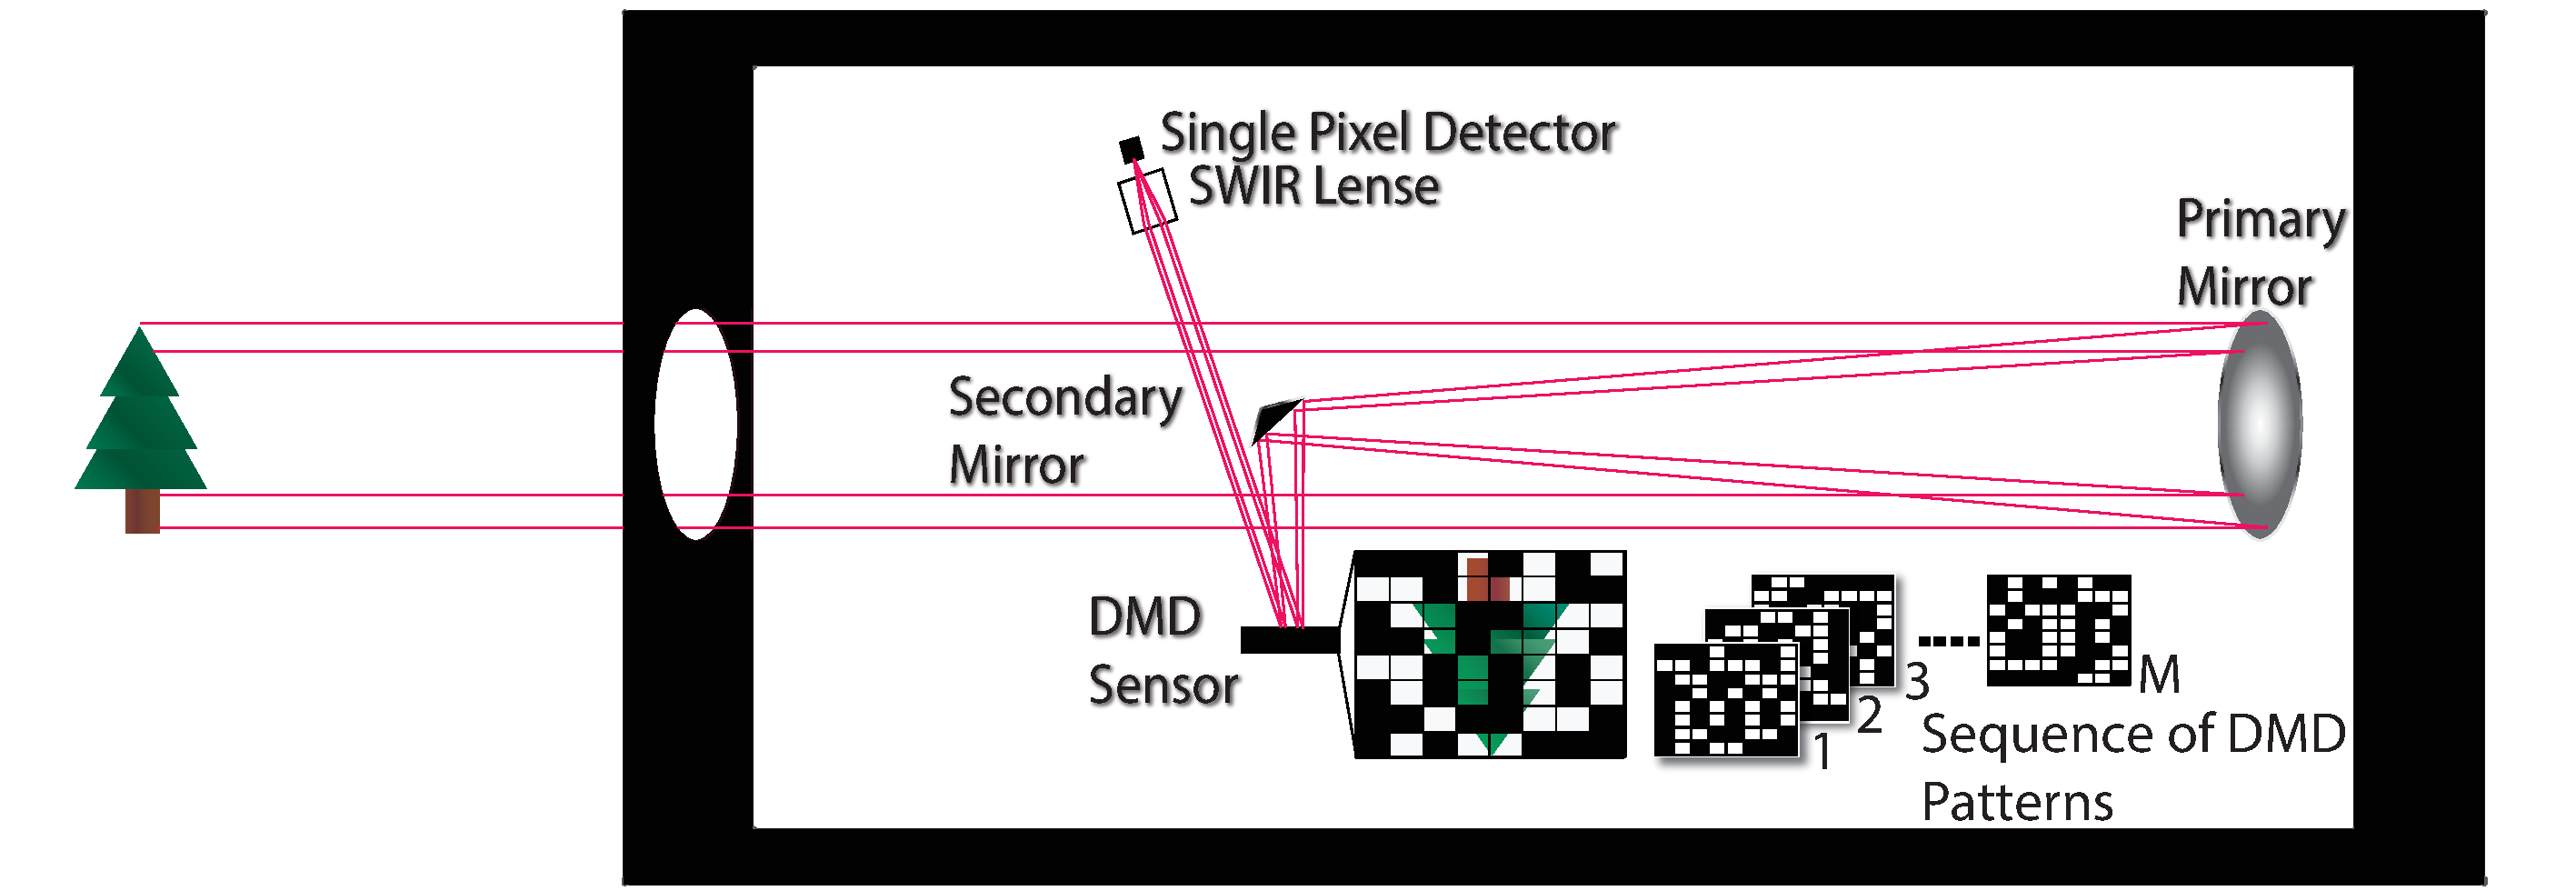
\includegraphics[width = \linewidth]{gfx/System_gif.eps}
	\caption{System overview}
	\label{fig:system_overview}
\end{figure}	

To connect the architecture with the math from CS it can be interpreted as, the light from the scene which is focused on the DMD is the desired signal $\mathbf{x}$, the image. The DMD can individually set each mirror the ether direct the light from each 'pixel' to the single pixel sensor or dump the light i.e a spatial light modulator (SLM). The DMD sets a pattern of pixel of intress which is a measurement matrix $\Phi_m$ to be summarized in the single pixel sensor $y_m$ as a measurement. One measurement is the inner product of a measurement matrix and the signal, $\Phi_m \times x = y_m$. To complete a full measurement the process is repeated with different measurement matrices set on the DMD to the full undetermined linear system $ \mathbf{y} = \mathbf{\Phi}\mathbf{x}$.

\subsection{Measurement matrix \& reconstruction}
How is the measurement matrix chosen? As told before the measurement matrix needs to be incoherent with the sparse transform and the DMD can only direct the light or not which mathematically is ether a zero or a one. The research tells that for example a i.i.d. Gaussian distribution with equal probability of a zero or one will with high probability be incoherent with a natural image scene. But how about the first constraint that the signal $\mathbf{x}$ needs to be sparse or compressible in some basis? Often natural images is not sparse in the spatial domain unless the scene is for example the night sky, well a good property of CS that the scene can be transformed to an other basis like this,

\begin{equation}
\label{eq:CS_1}
\mathbf{y} = \mathbf{\Phi} \mathbf{x} \Leftrightarrow \mathbf{y} = \mathbf{\Phi} \mathbf{\Psi} \mathbf{\Theta},
\end{equation}

where $\mathbf{\Psi}$ is a sparsitfying basis for example to the DCT or Wavelet basis. And $\mathbf{\Theta}$ is the coefficients vector which is more sparse then the spatial coefficient vector $\mathbf{x}$. And the transformation will not compromise the incoherence between the reconstruction matrix $A = \Psi\Phi$ and the coefficients $\Theta$ in the new basis. This means that the signal $\mathbf{x}$ will be reconstructed with optimization in a more sparse basis $\Theta$ and then transformed back to the spatial domain.\\[0.1in]

What is special about CS is not just how the problem is presented but also how to solve it. It is known that an undetermined linear system has infinite many solution so how does the signal get recovered? CS exploit the characteristics of the signal $x$ which is known to be sparse in some basis. With for example $\ell_1$ optimization,

\begin{equation}
\label{eq:l1_1}
\widehat{\mathbf{\Theta}} = \text{arg min} ||\mathbf{\Theta} ||_{\ell_1} \text{ subject to } \mathbf{\Phi} \mathbf{\Psi} \Theta = y,
\end{equation}    

which means that $\ell_1$ optimization minimizes the non zero elements of $\Theta$ and can exactly reconstruct a K-spares vector or approximate a compressible vector. The exact recovery can be accomplished with high probability using $M \geq \mathcal{O}(K\text{log}(N/K))$ measurements. This is why CS is powerful, it enables sub-Nyquist measurements with exact recovery in the noiseless case which can be approximated in real applications.\\[0.1in]

In the compressed imaging case where noise is present an other optimization algorithm has shown to be more successful at recovering images: total variation. Total variation regularization minimizes the magnitude of the gradient in the image and doing so it preserve edges and piece-wise constant structure in the image which is desired.     

 
\subsection{Motivation}
Why would a SPC be beneficial to a conventional camera? The SPC has more components and several measurements have to be made over time while a regular camera measures all pixels on the sensor at the same time, and the reconstruction shifts burden to the processor. There are two major reasons why a SPC is of interest, it is not to compete with the conventional cameras in the visual spectrum where cameras in all price ranges and quality already exist and are relative cheap to build. The focus lies in more exotic spectrum of light like SWIR or Terahertz (X-ray) wavelengths where the image sensors are hard to build which brings up cost and the ability to create high resolution sensors. With CS and the SPC architecture manufacturing cost can be significantly reduced while the image resolution increases. For example a state of the art SWIR camera cost about half a million SEK which can be reduced by a factor of 100 with a SPC with the same resolution. 

\subsection{Aim} 
What image quality can be achieved in natural images captured with a single pixel camera in daylight using state of the art methods?  


\subsection{Research questions} 
\label{sec:RQ}
\begin{itemize}
    \item How can the quality of images reconstructed by CS or a SPC be evaluated?
    \item What is the state of the art method to capture and reconstruct images using a SPC architecture?
    \item What image quality is achieved using state of the art methods applied to the SPC?
\end{itemize}

\subsection{Limitations}
\begin{itemize}
    \item The SPC provided by FOI is used and only minor changes can be made.
    \item The SPC is stationary at FOI and images can only be captured from that building.
    \item The reconstruction algorithm will not be developed in this thesis therefore free to use algorithms needs to be found.
\end{itemize}



\subsection{Thesis outline}
In this thesis the most important and inspirational articles will be presented with a small description in section~\ref{sec:related_work} \textit{Related work}. Section~\ref{sec:method} \textit{Method} presents a thorough review of the hardware, sensing- and reconstruction- method and the complete image capturing chain including pre- and post- processing. The method section includes essential compressive sensing and imaging theory, this section also present the evaluation techniques used in the result. Section~\ref{sec:Evaluation} \textit{Results} is divided into two categories, \textit{simulated results} and \textit{SPC results} where the same evaluation technique is performed on simulated and SPC images respectively in order to draw conclusions of the different parts of the chain. The results is followed by \textit{Discussion} and \textit{Conclusion \& Future Work} in section~\ref{sec:discussion} and \ref{sec:conclusions_and_fw} respectively. 
